\documentclass[border=6pt]{standalone}
\usepackage{pgfplots}
\pgfplotsset{compat=1.18}
\usepackage{xcolor}
\definecolor{bar}{HTML}{2A78D6}
\definecolor{top}{HTML}{EB6834}
\definecolor{surface}{HTML}{FCFCFB}
\definecolor{ink}{HTML}{0B0B0B}
\definecolor{muted}{HTML}{52514E}
\definecolor{gridc}{HTML}{E8E7E3}
\begin{document}
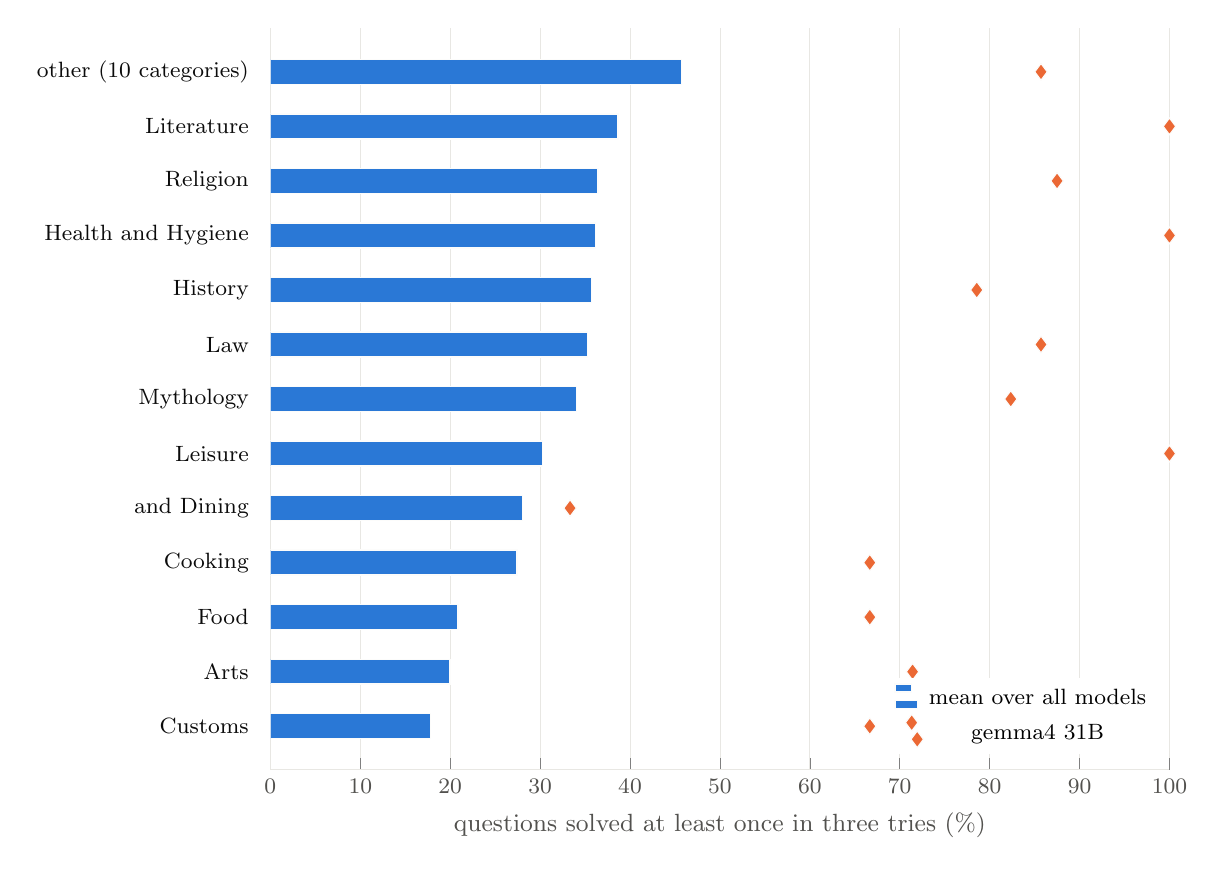
\begin{tikzpicture}
\begin{axis}[
  width=13cm, height=11cm, xbar, bar width=9pt,
  xlabel={questions solved at least once in three tries (\%)},
  xlabel style={font=\small, color=muted},
  tick label style={font=\footnotesize, color=muted},
  xmin=0, xmax=100, ymin=-0.8, ymax=12.8,
  ytick={0,1,2,3,4,5,6,7,8,9,10,11,12},
  yticklabels={Customs,Arts,Food, Cooking, and Dining,Leisure,Mythology,Law,History,Health and Hygiene,Religion,Literature,other (10 categories),Clothing,Geography},
  ytick style={draw=none},
  yticklabel style={font=\footnotesize, color=ink},
  xmajorgrids, grid style={gridc, line width=0.3pt},
  axis line style={gridc}, axis x line*=bottom, axis y line*=left,
  legend style={draw=none, font=\footnotesize, at={(0.99,0.02)}, anchor=south east},
]
\addplot[fill=bar, draw=surface, line width=0.5pt] coordinates {(17.78,0) (20.00,1) (20.89,2) (27.41,3) (28.05,4) (30.30,5) (34.02,6) (35.24,7) (35.71,8) (36.14,9) (36.46,10) (38.67,11) (45.71,12)};
\addlegendentry{mean over all models}
\addplot[only marks, mark=diamond*, mark size=3pt, mark options={fill=top, draw=surface}] coordinates {(66.67,0) (71.43,1) (66.67,2) (66.67,3) (33.33,4) (100.00,5) (82.35,6) (85.71,7) (78.57,8) (100.00,9) (87.50,10) (100.00,11) (85.71,12)};
\addlegendentry{gemma4 31B}
\end{axis}
\end{tikzpicture}
\end{document}
